\documentclass[a4paper]{scrartcl}
\usepackage[utf8]{inputenc}
\usepackage[english]{babel}

\usepackage{amsmath}
\usepackage{amsfonts} % for mathbb for instance
\usepackage{mathtools}
\usepackage[amsmath, amsthm, framed, thmmarks]{ntheorem}

% specifics about the pdf
\usepackage[english]{babel}
\usepackage[pdftex]{graphicx}
\usepackage[pdftex,bookmarks,colorlinks,pdffitwindow]{hyperref}

\usepackage{multicol}  
%\usepackage[rflt]{floatflt}  
\usepackage{epsfig} 
%\usepackage{qtree} 
\usepackage{url}

% PDF Import support
\usepackage{pdfpages}
% Support for PDF scaling
\usepackage{graphicx}
% Algorithmen
\usepackage{algorithmic}
\usepackage{algorithm}
\usepackage{listings} 
% \lstset{numbers=left, numberstyle=\tiny, numbersep=5pt} 
\lstset{
	basicstyle=\ttfamily\scriptsize\mdseries,
	keywordstyle=\bfseries\color{blue},
	identifierstyle=,
% 	stringstyle=\itshape\color{red},
	numbers=left,
	numberstyle=\tiny,
	stepnumber=10,
	breaklines=true,
	frame=none,
	showstringspaces=false,
	tabsize=4,
% 	backgroundcolor=\color{gray},
% 	morecomment=[s][\color{green}]{/+}{+/},
	commentstyle=\color{gray},	
	captionpos=b,
	float=htbp,
}
% math packages


% redefine greek letters
\renewcommand{\phi}{\varphi}
\renewcommand{\epsilon}{\varepsilon}

% shortcuts in math mode
\newcommand{\bs}{\boldsymbol}
\newcommand{\mc}{\mathcal}
\newcommand{\ds}{\displaystyle}
\DeclarePairedDelimiter\absimpl{\lvert}{\rvert}
\DeclarePairedDelimiter\normimpl{\lVert}{\rVert}
\newcommand{\abs}[1]{\absimpl*{#1}}
\newcommand{\norm}[1]{\normimpl*{#1}}
\newcommand{\argmax}{\operatorname*{arg\,max}}
\newcommand{\argmin}{\operatorname*{arg\,min}}

% number sets
\newcommand{\R}{\mathbb{R}}
\newcommand{\Z}{\mathbb{Z}}
\newcommand{\N}{\mathbb{N}}
\newcommand{\Q}{\mathbb{Q}}
\newcommand{\C}{\mathbb{C}}
\newcommand{\F}{\mathbb{F}}
\newcommand{\LL}{\mathcal{L}}
\newcommand{\powerset}{\mathcal P}
\newcommand{\normal}{\mathcal N}

% probabilities
\newcommand{\Prob}[1]{\operatorname{Pr}\left[#1\right]}
\newcommand{\Ex}[1]{\mathbb{E}\left[#1\right]}

% misc
\newcommand{\bigO}[1]{\mc O\left(#1\right)} % big-o notation

\newcommand{\nop}[1]{} % temporarily remove from output

% remove the paragraph indentation
 \setlength{\parindent}{0in}

\author{Pascal Spörri\\pascal@spoerri.io}
\title{Extended CIL Summary\\ FS 2013\\ }
%\thanks{Licence: Creative Commons Attribution-Share Alike 3.0 Unported (\url{http://creativecommons.org/licenses/by-sa/3.0/})}}
\date{\today}

\begin{document}
\maketitle
This summary is based on the course slides of the Computational Intelligence Lab slides\footnote{\url{http://cil.inf.ethz.ch}} from spring semester 2013.
\newpage
\tableofcontents

\part{Dimensionality Reduction}
Select the \emph{most interesting} dimensions. 

\section{Intrinsic Dimensionality}
\subsection*{Pairwise Distances}
Assume components of data $x=(x_1,\ldots,x_D)^T \in \R^D$ are i.i.d. Gaussian distributed:
\begin{align*}
    x_d \sim \normal(0,1) \implies x_d - y_d \sim \normal(0,2).
\end{align*}
Using $\chi^2$-distribution:
\begin{align*}
    {1\over 2}(x_d-y_d)^2 \sim \chi^2(1),
\end{align*}
and extending to $D$ dimensions:
\begin{align*}
    {1\over 2} \sum_{d=1}^D (x_d-y_d)^2 \sim \chi^2(D) = \Gamma\left( {D\over 2}, 2\right)\\
    \text{Recall: } \forall z,k, \theta > 0,\ \Gamma(z;k,\theta) = {\theta^k\over \Gamma(k)} y^{k-1} e^{-\theta z} 
\end{align*}
Hence, the dimension-normalised squared distance is:
\begin{align*}
    {1\over D} \sum_{d=1}^D (x_d-y_d)^2 \sim \Gamma\left({D\over 2}, {4\over D}\right)
\end{align*}
is Gamma distributed with mean $2$ and variance ${8 \over D}$. 

$\Gamma\left({D\over 2}, {4\over D}\right)$  tends towards normality with shrinking width for large $D$. Therefore, most points have \emph{constant} pairwise distances in this limit.

\section{Principal Component Analysis}
Objectives of PCA:
\begin{enumerate}
\item Minimise error $\norm{x_n-\tilde{x}_n}$ of point $x_n$ and its approximation $\tilde x_n$.
\item Reveal "interesting" information: maximise \emph{variance}.
\end{enumerate}
Both objectives are show to be formally equivalent.

Consider a set of observations $\{x_n\},\ n=1, \ldots, N$ and $x_n \in \R^D$.
\begin{description}
\item[Goal] Project data onto $K<D$ dimensional space while maximising variance of the projected data.
\item[For $\mathbf{K=1}$]  Define direction of projection as $u_1$. Set $\norm{u_1}_2 =1$ (only the direction of the projection is important.
\end{description}
\subsection{Statistics of Projected Data}
\paragraph{Original Data}
\begin{description}
\item[Mean] is given by the sample mean $\bar x$.
\item[Covariance] of the Data:
\begin{align*}
    \Sigma   = {1\over N} \sum_{n=1}^N (x_n - \bar x)(x_n - \bar x)^T
\end{align*}
\end{description}
\paragraph{Projected Data}
\begin{description}
\item[Mean] is given by: $u_1^T\bar x$.
\item[Variance] is given by:
\begin{align*}
    {1\over N} \sum_{n=1}^N \left\{ u_1^T x_n-u_1^T \bar x\right\}^2 
        &= {1\over N} \sum_{n=1}^N \left\{u_1^T (x_n-\bar x)\right\}^2\\
        &= {1\over N} \sum_{n=1}^N u_1^T (x_n - \bar x)(x_n-\bar x)^T u_1\\
        &= u_1^T \Sigma u_1.
\end{align*}
\end{description}

\subsection{Maximisation Problem}
These statistics now can be fed into a maximisation problem:
\begin{align*}
    \max_{u_1}\ u_1^T \Sigma u_1
\end{align*}
such that $\norm{u_1}_2 = 1$.

Writing the Lagrangian results in in:
\begin{align*}
    \mathcal L:= u_1^T \Sigma u_1 + \lambda_1(1-u_1^Tu_1). 
\end{align*}
Setting ${\delta \over \delta u_1}\mathcal L \overset{!}{=} 0$ results in:
\begin{align*}
    \Sigma u_1 = \lambda_1 u_1
\end{align*}

We observe that $u_1$ is an \emph{eigenvector} of $\Sigma$ and $\lambda_1$ it's associated \emph{eigenvalue}. Furthermore $\lambda_1$ is also the variance of the projected data:
\begin{align*}
    \lambda_1 = u_1^T \Sigma u_1
\end{align*}
\subsubsection{Second principal direction}
The second principal direction can be obtained by maximising the variance $u_2^T \Sigma u_2$, subject to $\norm{u_2}_2 = 1$ and $u_2^Tu_1 = 0$:
\begin{align*}
    \mathcal L = u_2^T \Sigma u_2 + \lambda_2\left( 1- u_2^Tu_2\right) +\nu \left(u_2^Tu_1\right).
\end{align*}
The maximum i found by setting ${\delta \mathcal L \over \delta u_2} \overset{!}{=} 0$:
\begin{align*}
    2\Sigma u_2 - 2\lambda_2 u_2+\nu u_1 = 0.
\end{align*}
Because of the orthogonality between $u_2$ and $u_1$ we observe that $u_2$ contains no component of $u_1$ and hence $\nu = 0$. We get:
\begin{align*}
    \Sigma u_2 = \lambda_2 u_2.
\end{align*}
We observe that $u_2$ is an eigenvector of $\Sigma$ with the second largest eigenvalue of $\lambda_2$.
\subsection{Solution: Eigenvalue Decomposition}
Hence we see that the eigenvalue decomposition of the covariance matrix
\begin{align*}
    \Sigma = U\Lambda U^T
\end{align*}
contains all relevant information. 

For a projection space of size $K\leq D$ we choose the $K$ eigenvectors $\{u_1,\ldots, u_k\}$ with the largest associated eigenvalues $\{\lambda_1, \ldots,\lambda_2\}$.

\subsection{Error Formulation}
We define an \emph{orthonormal} basis $\{u_d\}$, $d=1,\ldots, D$ of $\R^D$. The scalar projection of $x_n$ onto $u_d$ (magnitude) is given by:
\begin{align*}
    z_{n,d} = x_n^Tu_d.
\end{align*}
The associated projection onto $u_d$ amounts to $z_{n,d}u_d$. Therefore, each data point can be represented in the basis by:
\begin{align*}
    x_n = \sum_{d=1}^D z_{n,d}u_d=\sum_{d=1}^D\left(x_n^Tu_d\right) u_d.
\end{align*}

\emph{Restricted representation} using $K<D$ basis vectors can be written as:
\begin{align*}
\tilde x_n = \sum_{d=1}^K a_{n,d}u_d + \sum_{d=K+1}^D b_d u_d,
\end{align*}
where $b_d$ does not depend on the data point $x_n$.

The approximation error can be represented by:
\begin{align*}
 J(\{a_{n,d}\}, \{ b_d\}) &= {1\over N} \sum_{n=1}^N \norm{x_n-\tilde x_n}_2^2\\
\text{Minimisation of $J$ w.r.t.} a_{n,d} &= x_n^T\\
\text{Minimisation of $J$ w.r.t.} b_d &= \bar x^T u_d
\end{align*}
The displacement can be obtained by resubsittuing $a_{n,d}$ and $b_d$:
\begin{align*}
x_n - \tilde x_n = \sum_{d=K+1}^D \left\{\left(x_n-\bar x\right)^Tu_d\right\}u_d.
\end{align*}
We observe that the displacement vector is orthogonal to the principal space!

Resubstituting the displacement into the error criterion leads to:
\begin{align*}
    J= {1\over N} \sum_{n=1}^N \sum_{d=K+1}^D \left(x_n^T u_d - \bar x^T u_d\right)^2 = \sum_{d=K+1}^D u_d^T \Sigma u_d
\end{align*}

\subsection{Matrix viewpoint}
The data can be represented as matrix:
\begin{align*}
    X= [x_1,\ldots, x_n,\ldots, x_N]
\end{align*}
The corresponding zero-centered data is:
\begin{align*}
    \bar X = X-M,
\end{align*}
where $M=\underbrace{[\bar x, \ldots, \bar x]}_{N\ \text{times}}$.

Compute the projection of $\bar X$ on $U_k = [u_1,\ldots, u_K]$  with:
\begin{align*}
    \underbrace{\bar Z_K}_{K\times N} = 
        \underbrace{U_K^T}_{K\times D} \cdot \underbrace{\bar X}_{D \times N}.
\end{align*}

To approximate $\bar X$, we return to the original basis:
\begin{align*}
    \tilde{\bar X} = U_K\cdot \bar Z_K.
\end{align*}

For $K=D$  we obtain a perfect reconstruction.

\subsection{Computation}
First compute the \emph{empirical mean}:
\begin{align*}
\bar x = {1\over N} \sum_{n=1}^N x_n
\end{align*}
Then \emph{center the data} by subtracting the mean from each sample:
\begin{align*}
\bar X = X-M,
\end{align*}
where $M=\underbrace{[\bar x, \ldots, \bar x]}_{N\ \text{times}}$.
Now compute the \emph{Covariance matrix}:
\begin{align*}
\Sigma = {1\over N} \sum_{n=1}^N (x_n-\bar x)(x_n-\bar x)^T = {1\over N} \underbrace{\bar X\bar X^T}_{\text{Scatter Matrix }\mathbf S}.
\end{align*}
$\Sigma$ is \emph{symmetric}. 

Now the \emph{Eigenvalue decomposition} can be computed:
\begin{align*}
\Sigma = U\Lambda U^T,
\end{align*}
where $\Lambda = diag[\lambda_1, \ldots, \lambda_D]$, such that $\lambda_1 \geq \lambda_2 \geq \ldots \geq \lambda_D$ with orthonormal eigenvectors.

\begin{description}
\item[Transformation] the data can be transformed on to the new basis of $K$ dimensions:
\begin{align*}
    \tilde{\bar Z} = U_K^T \bar X,
\end{align*}
$\bar Z \in \R^{K\times N}$: We obtain a dimension reduction of the data.
\item[Reconstruction] Go back to the original basis by computing
\begin{align*}
    \tilde{\bar X} &= U_K \bar Z\\
    \tilde X &= \tilde{\bar X}+M
\end{align*}


\end{description}




\section{Singular Value Decomposition}

\subsection{Introduction}
The \emph{Singular Value Decomposition} (SVD) is a widely used technique to decompose a matrix into several component matrices exposing many of the useful and interesting properties of the original matrix
like rank, null-space, orthogonal basis of column and row space. 

Every rectangular, real or complex matrix $S$ has an SVD decomposition into a set of three matrix factors.

Let $A$ be any real $M$ by $N$ matrix, $A \in \R^{M\times N}$ , then $A$ can be decomposed as $A=UDV^T$:
\begin{figure}[H]
    \centering
    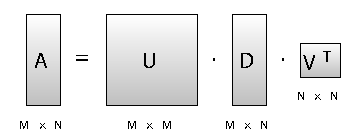
\includegraphics[width=0.75\textwidth]{img/svd_decomposition}
\end{figure}
\begin{itemize}
    \item $U$ is an $M\times M$ orthogonal matrix, $U^TU=I$
    \item $D$ is an $M\times N$ diagonal matrix
    \item $V^T$  is an $N\times N$ orthogonal matrix, $V^TV=I$ 
\end{itemize}
\subsection{Singular values}
The elements of $D$ are only non-zero on the diagonal and are called the \emph{singular values}. By convention, the order of the singular vectors is determined by the \emph{high-to-low} sorting of singular values, with the highest singular value in the upper left index of the $D$ matrix.
The first $r$ columns of $U$ are called \emph{left singular vectors}, they form an orthogonal basis for the space spanned by the columns of the original matrix $A$.

Similarly the first $r$ rows of $V^T$ are the \emph{right singular vectors}, they form an orthonormal basis for the row space of $A$.

SVD provides an explicit representation of the range and null-space of a matrix $A$.
\begin{itemize}
\item The right side singular vectors corresponding to vanishing singular values of $A$, span the null space of $A$:
\begin{align*}
d_i = 0 \quad \implies \quad Av_i = 0 \quad \implies \quad v_i \in Null(A).
\end{align*}
\item The left singular vectors corresponding to the non-zero singular values of $A$ span the range of $A$.
\end{itemize}
As a consequence, the rank of $A$ equals the number of non-zero singular values (= the number of non-zero elements in $D$).
\begin{align*}
Rank(A) = \# d_i > 0.
\end{align*}
\subsection{Closest Rank-$k$ Matrix}
Let the SVD of $A \in \R^{M\times N}$  be given by $A=UDV^T$. If $k<r = Rank(A)$ and
\begin{align*}
    A_k = \sum_{i=1}^k d_i u_i v_i^T.
\end{align*}
Then 
\begin{align*}
    \min_{Rank(B)=k} \norm{A-B}_2 = \norm{A-A_k}_2.
\end{align*}
This means that $A_k$ is the closest $Rank(k)$ approximation to $A$ in the Eculidean matrix norm sense hence:
\begin{align*}
    \norm{A-A_k}_2 = d_{k+1}.
\end{align*}

\subsection{Properties}
The columns of $U$ are the eigenvectors of $AA^T$. This claim can be verified using the SVD decomposition:
\begin{align*}
    AA^T = UDV^T VDU^T = UD^2U^T.
\end{align*}
Similarly the rows of $V^T$ (or columns of $V$) are the eigenvectors of $A^TA$ as:
\begin{align*}
    A^TA = VDU^T UDV^T = VD^2V^T.
\end{align*}



\newpage
\part{Clustering}

\section{Introduction}
A set of datapoints in a $d$-dimensional Euclidean space is given.
\begin{description}
    \item[Aim] The aim is to find a \emph{meaningful partition} of the data; i.e. label each data point with a unique value $\{1,\ldots, k\}$.
    \item[Objective] The partition should group together similar data points, while the different groups/clusters should be as dissimilar as possible from each other.
    \item This way we can uncover similarities between data points and give rise to data compression schemes.
\end{description}


\subsection{Problem}
Consider $N$ data points in a $D$-dimensional space. Each data vector is denoted by $x_n$, $n=1,\ldots,N$. Our goal is to partition the data set into $K$ clusters: Find vectors $u_1, \ldots, u_K$ that represent the centroid of each cluster.

A datapoint $x_n$ belongs to cluster $k$ if the Euclidean distance between $x_n$ and $u_k$ is smaller than the distance to any any other centroid.

Mathematically, the clustering problem defines a mixed discrete continuous optimisation problem. 

\subsubsection{The Cost Function of Vector Quantisation}
\begin{description}
    \item[Objective] Minimise the cost function
        \begin{align*}
            J(U,Z) = \norm{X-UZ}_F^2 = \sum_{n=1}^N\sum_{k=1}^K z_{k,n} \norm{x_n-u_k}_2^2
        \end{align*}
        where
        \begin{align*}
            X &= [x_1,\ldots, x_N] \in \R^{D\times N}\\
            U &= [u_1,\ldots, u_K] \in \R^{D\times K}, &\text{centroids}\\
            Z &\in \{0,1\}^{K\times N}, &\text{assignments}
        \end{align*}
        with $\sum_k z_{k,n} = 1 \forall n$ i.e.,  one element per columns set to $1$.
\end{description}
Assignment notation:
\begin{description}
    \item[Assignment Notation]: Vector $\hat z \in \{1,\ldots,K\}^N$ indicating for each data point to which cluster index it is assigned:
    \begin{align*}
        \hat z = \begin{pmatrix}
                    2\\ 3\\ 4\\ 2 \\ 2\\ 1
                 \end{pmatrix}
    \end{align*}
    \item[Matrix Notation]: The matrix $Z\in \{0,1\}^{K\times N}$ with only one non-zero entry per column, assigns data points to clusters:
    \begin{align*}
        Z &= \begin{pmatrix}
                 0&0&0&0&0&1\\
                 1&0&0&1&1&0\\
                 0&1&0&0&0&0\\
                 0&0&1&0&0&0
             \end{pmatrix}
    \end{align*}
\end{description}

\section{$K$-Means}
\subsection{Overview}

The algorithm alternates between two steps:
\begin{itemize}
    \item \emph{Assigning data points} to clusters
    Let $k^*(x_n)$ denote the cluster index with the minimal distance between a cluster centroid and the data point $x_n$:
    \begin{align*}
    k^*(x_n) &=\argmin_k \left\{ \norm{x_n-u_1}_2^2,\ldots, \norm{x_n-u_k}_2^2,\ldots,\norm{x_n-u_K}_2^2 \right\}
    \end{align*}

    \item \emph{Updating the cluster centroids} based on all the data points assigned to it. Compute the mean/centroid of a cluster that can be written as:
    \begin{align*}
        u_k = {\sum_{n=1}^N z_{k,n} x_n \over \sum_{n=1}^N z_{k,n} }\quad \forall k,\ \ k\in \{1,\ldots,K\}
    \end{align*}
\end{itemize}

\subsection{Algorithm}
\begin{enumerate}
\item Initiate with a random choice of $u_1^{(0)}, \ldots, u_K^{(0)}$ (or let $u_1^{(0)}, \ldots, u_K^{(0)}$ equal data points from the set). Set $t=1$.
\item \textbf{Cluster assignment.} Solve $\forall n$:
    \begin{align*}
        k^*(x_n) &=\argmin_k \left\{ \norm{x_n-u_1^{(t)}}_2^2,\ldots, \norm{x_n-u_K^{(t)}}_2^2 \right\}.
    \end{align*}
    Then, $z_{k*(x_n),n}^{(t)} = 1$ and $z_{j,n}^{(t)} =0\ \forall j\neq k,\ \ j=1,\ldots, K$.
\item \textbf{Centroid update} 
    \begin{align*}
        u_k^{(t)} = {\sum_{n=1}^N z_{k,n}^{(t)} x_n \over \sum_{i=1}^N z_{k,n}^{(t)}}\ \forall k,\ k\in\{1,\ldots,K\}
    \end{align*}
\item Increment $t$. Repeat step $2$ until $\norm{u_k^{(t)}-u_k^{(t-1)}}_2^2 < \varepsilon\ \forall K$ ($0<\varepsilon << 1$) or until $t=t_\text{finish}$.  
\end{enumerate}
Aspects:
\begin{itemize}
    \item The computational cost of each iteration is $\bigO{KN}$.
    \item Convergence is guaranteed
    \item Optimises a \emph{non-convex} objective. Hence only a local minimum can be guaranteed.
    \item Can be used to compress data: store only the centroids and the assignments of data point to clusters.
\end{itemize}
Problems:
\begin{itemize}
\item Non-convex objective, local minima and sensitive to initialisations.
\item Not appropriate for non-Euclidean data $\mapsto$ need to use other distances.
\item The optimal number of clusters $K$ is unknown: One has to find a balance between total compression $(K=1)$ and no loss of information $(K=N)$.
\end{itemize}

\subsection{Stability}
\subsubsection{High-Level Stability test}
The following is a high-level stability test for a given set of data points and a given number of clusters:
\begin{enumerate}
    \item Generate perturbed versions of the set for example by adding noise or drawing sub-samples.
    \item Apply the clustering algorithm on all versions.
    \item Compute pair-wise distances between all clusterings (using some distance measure).
    \item Compute the \emph{instability} as the mean distance between all clusterings.
\end{enumerate}
Repeat this for different numbers of clusters and choose the one that minimises the instability.
\subsubsection{Distance between Clusterings}
For two clusterings $C$ and $C'$ that are defined on the same data points we compute the distance between clusterings $d$ in the following procedure:
\begin{enumerate}
    \item Compute the distances between the two clusterings by counting points on which the two clusterings agree or disagree.
    \item Repeat over all permutations of the cluster labels (since the same cluster might be sometimes labeled $1$ and sometimes $2$ etc...).
    \item Choose the permutation with minimal distance and the corresponding distances is $d$.
\end{enumerate}
In other words,
\begin{align*}
    d = \min_\pi \norm{Z-\pi(Z')}_0
\end{align*}
where $\pi(Z')$ is one of the possible row permutations of $Z'$ and $\norm{Z}_0$ denotes the cardinality of $Z$.
If two clusterings are defined on different data sets but many points overlap, we use only these for comparison, otherwise, a mapping from one domain to the other is required.

\subsubsection{Calculation of Stability}
The rate of inconsistent data items $r$ is computed as follows"
\begin{enumerate}
    \item Cluster data sets $X$, $X'$ to infer assignments $Z$, $Z'$.
    \item Train a classifier $\phi$ on $(X,Z)$ to transfer the clustering results $Z$ on $X$ to $X'$.
    \item Apply $\phi$ on $X'$ and compare the optimally permuted output with $Z'$:
    \begin{align*}
        r:= {1\over N} \min_{\pi \in \mathbb S_K} \left\{ \sum_{i=1}^N \mathbb I_{\{ \pi(\phi(x_i'))\neq\hat z_i' \}}\right\}.
    \end{align*}
The indicator function $\mathbb I_{\{p\}}$ is $1$ if predicate $p$ is true, and $0$ otherwise.

Minimisation of $\pi\in \mathbb S_K$ compensates for the permutation of the cluster numbers.
\end{enumerate}
The higher the number of clusters, the more difficult it is to have a small rate $r$ of inconsistent cluster assignments. Given $K$ clusters of equal size, a random assignment yields
\begin{align*}
    r_{rand} = {K-1\over K}.
\end{align*}
To be able to compare hypotheses with different $K$, relate $r$ to $r_{rand}$. The \emph{stability} is this defined as:
\begin{align*}
    stab := 1 - {r \over r_{rand}}.
\end{align*}
\begin{itemize}
    \item $stab=1$: No inconsistent assignments
    \item $stab=0$: Not better than a random assignment
\end{itemize}

\section{Clustering as Matrix Factorisation}
SVD is a class matrix factorisation technique according to which every matrix matrix can be decomposed into $X=UDV^T$. With $U\in \R^{D\times D}$, $D\in \R^{D\times N}$ and $V\in \R^{N\times N}$.
By setting $UD$ in the decomposition as $U$ and renaming $V^T$ to $Z$, we can write
\begin{align*}
    X= UZ.
\end{align*}

Approximating $X$ using the $K$ largest singular values we get a factorisation involving matrices of the same dimensionality as $K$-Means. 




\section{Mixture Models}
\subsection{Soft Clustering}
The term Soft clustering is ambiguous since it can refer to the algorithm or to the model:
\begin{description}
\item[Algorithmic] Soft $K$-Means: Instead of assigning a point to exactly one cluster. Consider assigning a probability that a data point belongs to a certain cluster. 
\item[Model relaxation]
\end{description}

\section{Multi-Assignment Clustering}

\subsection{Role-Based Access Control (RBAC)}
Given a \emph{user-permission} matrix $X\in \mathbb B^{D\times N}$, find
\begin{description}
\item[Roles] $U\in \mathbb B^{D\times K}$ and
\item[Assignments] $Z\in \mathbb B^{K\times N}$ 
\end{description}
with $\mathbb B=\{0,1\}$ such that
\begin{align*}
    X = U \otimes Z \quad \Leftrightarrow \quad x_{dn} = \bigvee_k [u_{dk} \land z_{kn}].
\end{align*}
\begin{itemize}
\item Each role defines a set of permissions
\item Users are assigned to a set of roles and get all permissions of these roles.
\end{itemize}

\subsubsection{Notation}
\begin{itemize}
\item $x_{dn} \in \{0,1\}$: Assignment of user $n$ to permission $d$.
\item $z_{kn} \in \{0,1\}$: Assignment of user $n$ to role $k$.
\item $u_{dk} \in \{0,1\}$: Assignment of permission $d$ to role $k$.
\item $\beta_{dk} \in [0,1]$: Probability of $u_{dk} = 0$.
\end{itemize}
\begin{figure}[H]
    \centering
    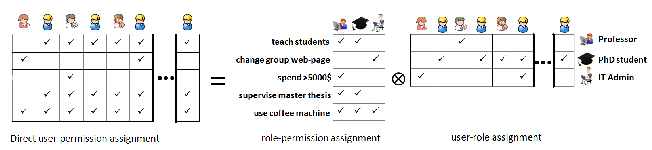
\includegraphics[width=\textwidth]{img/multi_assignment_rbac}
\end{figure}

\subsubsection{Evaluation Criteria}
For each role mining problem definition, there is a (set of) evaluation criteria:
\begin{itemize}
\item Matrix Reconstruction
\item Number of Sources
\item Inference Quality
\item Generalisation
\item Stability
\end{itemize}

\subsection{Binary Matrix Factorisation}
\emph{Min-Noise Approximation}: Given $K$, find the matrices $\hat U$, $\hat Z$ such that
\begin{align*}
    (\hat U, \hat Z) =\argmin_{U,Z} \norm{X-U\otimes Z}_1
\end{align*}
with $U\in \mathbb B^{D\times K}$ and $Z\in \mathbb B^{K\times N}$. This problem is also called \emph{approximate Boolean Matrix decomposition} and has the following properties:
\begin{itemize}
    \item \textbf{All} matrices are Boolean,
    \item It is a \emph{combinatorial optimisation problem},
    \item It is proven to be \emph{NP-hard} (reducible to set basis problem).
\end{itemize}
In contrast to recommender systems a the outputs $\hat U$ and $\hat Z$ are always binary.

\subsubsection{Rounded SVD}
\begin{enumerate}
    \item Compute the singular value decomposition
        \begin{align*}
            X=U\cdot S\cdot V^T
        \end{align*}
    \item Discard columns $K+1,\ldots,D$ of $U$ to get $U_{(K)}$.\\
          Discard rows $K+1,\ldots,N$ of $V$ to get $V_{(K)}$.
    \item Round the left and right singular vectors to get Boolean matrices $\hat U$ (roles) and $\hat Z$ (role assignments):
        \begin{align*}
            \hat U &= (U_{(K)} > t_U)\\
            \hat Z &= (V_{(K)} > t_V)
        \end{align*}
        where $t_U$ and $t_V$ are thresholds.
\end{enumerate}
The rounded continuous decomposition is a poor Boolean decomposition!

\subsubsection{$K$-means}
$K$-means partitions objects into disjoint groups (clusters) s.t. the average \emph{distance} between data and corresponding cluster prototypes is minimal. 
The standard objective function for $K$-means uses the \emph{Euclidean distance} measure:
\begin{align*}
    J(U,Z) = \norm{X-UZ}_2^2 = \sum_{n=1}^N \sum_{k=1}^K z_{kn} \norm{x_n - u_k}_2^2
\end{align*}
and centroids are updated via mean operation.

In order to use $K$-means for a Boolean decomposition the distance is adapted to use \emph{Hamming distance} (0-norm):
\begin{align*}
    J(U,Z) = \norm{X-UZ}_0 = \sum_{n=1}^N \sum_{k=1}^K z_{kn} \norm{x_n - u_k}_0
\end{align*}
The centroids $u_k$ are restricted to Boolean values and the centroid update step needs to be adapted:
\begin{align*}
    u_{dk} = \text{median}(\{x_{dn}|z_{kn} =1 \})\ \forall k\in \{1,\ldots,K\},\ \forall d \in \{1,\ldots, D\}
\end{align*}

$K$ can be found with cross-validation. $K$-means only yields \emph{disjoint clustering}, i.e. $Z$ matrix has only a single $1$ in each column. In RBAC however a user can have multiple role. 

\subsubsection{RoleMiner}
RoleMiner is a heuristic for role mining. Idea: A set of common permissions could potentially be a role. Roles are created by finding common sets of permissions between user.

Comes in two variants: \emph{CompleteMiner} and \emph{FastMiner}.

RoleMiner is very sensitive to noise:
\begin{itemize}
    \item If only a few individual bits are noisy, then the number of candidate roles gets much larger.
    \item The result is unstable: If the noise changes slightly, then the solution is completely different.
\end{itemize}

\subsubsection{DBPsolver}
DBPsolver approximately solves the \emph{Discrete Basis Problem}.
\paragraph{Discrete Basis Problem:} For a given Boolean matrix $X\in \mathcal B^{D\times N}$ and a number $K$ of basis vectors, find a Boolean matrix $U\in \mathcal B^{D\times K}$ and a Boolean matrix $Z\in \mathcal B^{K\times N}$ minimising 
\begin{align*}
    \norm{X-U\otimes Z}_F^2.
\end{align*}
The discrete basis problem and min-noise Role Mining problem are identical.

\subsubsection{Probabilistic Clustering}
\paragraph{Difficulties so far}
\begin{itemize}
 \item Searching in the full Boolean spaces has a \emph{too high complexity}.
 \item Restricting the Boolean search spaces \emph{ignores solutions}
 \item Searching solutions in continuous space and rounding \emph{produces poor results}.
 \item Search heuristics are prone to \emph{overfitting}
\end{itemize}

\paragraph{Modeling of RBAC} Computing a likelihood requires to design a probabilistic model $p(X|U,Z)$ for the generation process of the data $X$. This is the probability $X$ given the model, the cluster assignments $Z$, and the cluster centroids $U$.

\paragraph{Derivation I: One Object} For the simple case we consider one cluster per object:
\begin{align*}
\sum_k z_{kn} = 1, \qquad \forall n \in \{1, \ldots, N\}.
\end{align*}
$k_n$ is the cluster of object $n$: 
\begin{align*}
    k_{n} = \{ k\in \{1, \ldots, L\}| z_{kn} = 1\}.
\end{align*}
Consider on entry $x_{dn}$:\todo{WTF}
\begin{align*}
    p(x_{dn} = 0 | \beta_{d\cdot},z_{\cdot n}) = \beta_{dk_n}.
\end{align*}
Therefore:
\begin{align*}
    p(x_{dn} = 1 | \beta_{d\cdot},z_{\cdot n}) &=  1 - p(x_{dn} = 0 | \beta_{d\cdot},z_{\cdot n})\\
        &= 1-\beta_{dk_n}
\end{align*}

\paragraph{Derivation II: All objects} Objects are now independent given the parameters $Z$ and $U$. Thus:
\begin{align*}
    p(X|\beta,Z) &= \prod_{n=1}^N \prod_{d=1}^D p(x_{dn} = 1 | \beta_{d\cdot},z_{\cdot n})^{x_{dn}}\cdot p(x_{dn} = 0 | \beta_{d\cdot},z_{\cdot n})^{1-x_{dn}}\\
     &= \prod_{n,d} (1-\beta_{dk_n})^{x_{dn}} \beta_{dk_n}^{1-x_{dn}}
\end{align*}

\subsubsection{Multi-Assignment Clustering}
Compared to probabilistic clustering we don't restrict an object to one cluster.

One $x_{\cdot n}$ is generated by a \emph{set of clusters} $\mathcal L_n := \{k|z_{kn} = 1\}$. The resulting Boolean features are generated by \emph{disjunction} of the corresponding Boolean cluster centroids $u_{k,}$ (logical OR).
\begin{figure}[H]
    \centering
    
\includegraphics[width=0.8\textwidth]{img/multi_assignment_clustering}
    \caption{An object as the disjunction of the three clusters it belongs to.}
\end{figure}

\paragraph{Probabilistic view:} An object being generated by two clusters $k_1$, $k_2$ has probability $\beta_{dk_1}\beta_{dk_2}$ to have a $0$ at this dimension. 

Generally, an object $n$ belonging to the set of clusters $\mathcal L_n := \{ k|z_{kn} = 1\}$ has a probability $\beta_{\mathcal L_n} := \prod_{k\in \mathcal L_n} \beta_{dk}$ for a $0$ at dimension $d$.


In turn, it holds that $p(x_{dn}=1|z,\beta) = 1-\beta_{\mathcal L_n}$. Thus we get the following model:
\begin{align*}
    p(X|\beta, Z) = \prod_{n,d} \underbrace{\left(1-\prod_k \beta_{dk}^{z_{kn}} \right)^{x_{dn}} }_{\text{Noise component}} \underbrace{\left(\prod_k \beta_{dk}^{z_{kn}}\right)^{1-x_{dn}}}_{\text{Signal component}}
\end{align*}
\todo{Not sure about the component naming}

\subsubsection{Noise model for RBAC}

The deterministic RBAC generation of $X$:
\begin{align*}
    X = U\otimes Z \quad \Leftrightarrow\quad  x_{dn} = \bigvee_k [u_{dk} \land z_{kn}].
\end{align*}
Since this generation rule is not able to explain erroneous assignments in $X$ as noise we introduce a \emph{mixture noise model}:
\begin{align*}
    x_{dn} = (1-\xi_{dn})(U\otimes Z)_{dn} + \xi_{dn}\eta_{dn}
\end{align*}
where $\xi_{dn}$ is a binary noise indicator and $\eta_{dn}$ is a binary random variable.

\paragraph{Mixture Noise Model} Noise generation:
\begin{itemize}
    \item $\xi_{dn}$ indicates whether a bit is generated by $p_N (\xi_{dn}=1)$ or by $(U\otimes Z)_{dn}(\xi_{dn}=1)$. $\xi_{dn}$ is Bernoulli distributed:
    \begin{align*}
        p(\xi_{dn}|\varepsilon) = \varepsilon^{\xi_{dn}} (1-\varepsilon)^{1-\xi_{dn}},
    \end{align*}
    where $\varepsilon$ is the probability to choose a random bit.
    \item If the bits is noisy ($\xi_{dn}=1$), draw $\eta_{dn} = x_{dn}$ from
    \begin{align*}
        p_N(x_{dn}|r) = r^{x_{dn}} (1-r)^{1-x_{dn}},
    \end{align*}
    with $r$ being the probability that a noisy bit is $1$ ie. a user exceptionally gets a permission.
\end{itemize}
This can be modelled to a structure model:
\begin{align*}
    p_S(X|\beta, Z) = \prod_{n,d} \left( 1-\prod_k (\beta_{dk})^{z_{kn}}\right)^{x_{dn}} \left( \prod_k (\beta_{dk})^{z_{kn}}\right)^{1-x_{dn}},
\end{align*}
with $\beta_{dk}=p(u_{dk}=0)$.

This then can be combined with the noise model:
\begin{align*}
    p(X|Z, \beta, \xi, r) &= \prod_{n,d} p_N(x_{dn}|r)^{\xi_{dn}} p_S(x_{dn}|\beta_{d\cdot}, z_{\cdot n})^{1-\xi_{dn}}\\ 
    &= \prod_{n,d} \underbrace{\left( r^{x_{dn}}(1-r)^{1-x_{dn}}\right)^{\xi_{dn}}}_{x_{dn}\text{ generated by noise}}
    \underbrace{
        \left(\left[1-\prod_k (\beta_{dk})^{z_{kn}}\right]^{x_{dn}} 
            \left[ \prod_k(\beta_{dk})^{z_{kn}} \right]^{1-x_{dn}}
        \right)^{1-\xi_{dn}}
    }_{x_{dn}\text{ generated by roles}}.
\end{align*}

The $\xi_{dn}$ are unobservable (hidden) variables:
\begin{itemize}
\item They are unknown.
\item They are too many to be estimated.
\end{itemize}

We thus integrate the $\xi$ out of $p(X|Z,\beta, \varepsilon, \xi, r)$:
\begin{align*}
    p(X|Z,\beta,\varepsilon,r) = \sum_{\{\xi\}} p(X,\xi|Z,\beta, \varepsilon,r),
\end{align*}
where
\begin{align*}
    p(X,\xi|Z,\beta, \varepsilon, r) &=
        p(X|Z,\beta,\xi, r)p(\xi|\varepsilon)\\
        &= p(X|Z,\beta,\xi, r)\prod_{n,d}\varepsilon^{\xi_{dn}} (1-\varepsilon)^{1-\xi_{dn}}\\
        &= \prod_{n,d} \left(\varepsilon r^{x_{dn}} (1-r)^{1-x_{dn}}\right)^{\xi_{dn}}
            \left((1-\varepsilon)(1-\beta_{d,\mathcal L_n})^{x_{dn}}(\beta_{d,\mathcal L_n})^{1-x_{dn}}\right)^{1-\xi_{dn}}.
\end{align*}

\paragraph{Mixture Model:}
The likelihood function can thus be written as:
\begin{align*}
    p(X|Z,\beta,\varepsilon,r) &=
        \prod_{n,d} \left( \varepsilon r^{x_{dn}} (1-r)^{1-x_{dn}}+(1-\varepsilon)(1-\beta_{d,\mathcal L_n})^{x_{dn}} (\beta_{d,\mathcal L_n})^{1-x_{dn}} \right)\\
        &=  \prod_{n,d} \left(\varepsilon r + (1-\varepsilon)(1-\beta_{d,\mathcal L_n})\right)^{x_{dn}}
        \left(\varepsilon (1-r)+(1-\varepsilon)\beta_{d,\mathcal L_n}\right)^{1-x_{dn}}
\end{align*}
Parameters to estimate:
\begin{itemize}
    \item $Z$: user-role assignments.
    \item $\beta$: probabilities of role-permission assignments $U$ to be $0$.
    \item $\varepsilon$: noise probability.
    \item $r$: probability of noisy bits to be $1$.
\end{itemize}

This function requires a non-convex objective function to maximise the log-likelihood.

\newpage
\appendix
 
\part{Appendix}
\section{Matrix Definitions and Theorems}
\subsection{Norms}
A \emph{norm} is a function $\norm{\circ}: V \mapsto \R$ quantifying the size of a vector. It must satisfy
\begin{itemize}
    \item \emph{Positive scalability:}
    \begin{align*}
        \norm{a\cdot x} &= |a|\cdot \norm{x}.
    \end{align*}
    \item \emph{Triangle inequality}
    \begin{align*}
        \norm{x+y} \leq \norm{x} + \norm{y} \quad \forall x,y \in V.
    \end{align*}
    \item \emph{Separability}:
    \begin{align*}
        \norm{x} = 0 \ \implies \ x=0.
    \end{align*}
\end{itemize}
\subsubsection{Vector norms}
\begin{description}
    \item[$\mathbf{p}$-norms] The most commonly used matrix norms are $p$-norms.
        \begin{align*}
            \norm{x}_p := \left(\sum_{i-1}^n |x_i|^p\right)^{1/p}
        \end{align*}
        for $p \in [1,\infty]$, where $|x_i|$ denotes the absolute value of coordinate $x_i$.
        
        A special case of the $p$ norm is the \emph{Eclidean norm}:
        \begin{align*}
            \norm{x}_2:= \sqrt{\sum_{i=1}^n x_i^2}.
        \end{align*}
    \item[$0$-norm] technically not really a norm is defined by:
        \begin{align*}
            \norm{x}_0 := \text{number of nonzero coordinates in $x$}.
        \end{align*}
\end{description}
\subsubsection{Matrix norms}
\begin{description}
    \item[$p$-norm] for matrices:
        \begin{align*}
            \norm{X}_p := \max_{x\neq 0} {\norm{Ax}_p \over \norm{x}_p}.
        \end{align*}
        A special case is the Euclidean or \emph{spectral norm}:
        \begin{align*}
            \norm{X}_2 = \sigma_\text{max} (X),
        \end{align*}
        the largest singular value of $X$.
    \item[Frobenius norm] is defined as:
        \begin{align*}
            \norm{X}_F := \sqrt{\sum_{i=1}^m \sum_{j=1}^n x_{ij}^2} = \sum_{i=1}^{\text{min}(m,n)} \sigma_i^2,
        \end{align*}
        where $\sigma_i$ are the singular values of $X$.
        
        
\end{description}

\subsection{Orthogonality}
\begin{description}
    \item[Orthogonal vectors] Two vectors in an inner product are orthogonal if their inner product is zero.
    \item[Orthonormal vectors] Orthogonal vectors that have unit length 1
    \item[Orthogonal matrix] An orthogonal matrix is a square matrix with real entries whose columns and rows are orthogonal unit vectors (i.e. orthonormal vectors).
    For orthogonal matrices it also holds that
    \begin{align*}
        A^T A= I \quad \implies \quad A^T = A^{-1}\ &\text{since,}\\
        (A^TA)_{i,j} &= a_i^Ta_j = 
            \begin{cases}
                1&i=j\\
                0&i\neq j
            \end{cases}
    \end{align*}

\end{description}


\end{document}
